% !TEX program = pdflatex
\chapter[Domain Names]{Domain Names, SSL, and Versioning\\\small{\textit{-- Charles, Justin, Benedict, Jacky}}}
\label{Chapter::Domain Names}
\index{Chapter!Domain Names}

% \section{Assignment Overview}
% This chapter documents how our group configured a custom domain, secured it with SSL, and connected it to an Overleaf instance hosted via DigitalOcean and GitHub Pages.  
% The work combines the DigitalOcean setup (completed by team members on macOS) with my GitHub Pages + SSL configuration.  
% Screenshots and command examples are provided for each major step.

%----------------------------------------------------
\section{Domain Registration}
\begin{enumerate}
    \item Our team registered the domain \url{https://latex.ssw590group11overleaf.me} using Namecheap.
    \item We received a free domain through our GitHub Student Developer pack and signed up at this website \url{https://nc.me}.
    \item We then hosted this domain using GitHub Pages.
    \item This domain was also linked to the Overleaf container we created using the DigitalOcean droplet.
\end{enumerate}
%  through the GitHub Student Developer Pack (free for one year).  
% The domain was verified, includes WHOIS privacy protection, and is configured to auto-renew.

% \begin{figure}[h!]
%     \centering
%     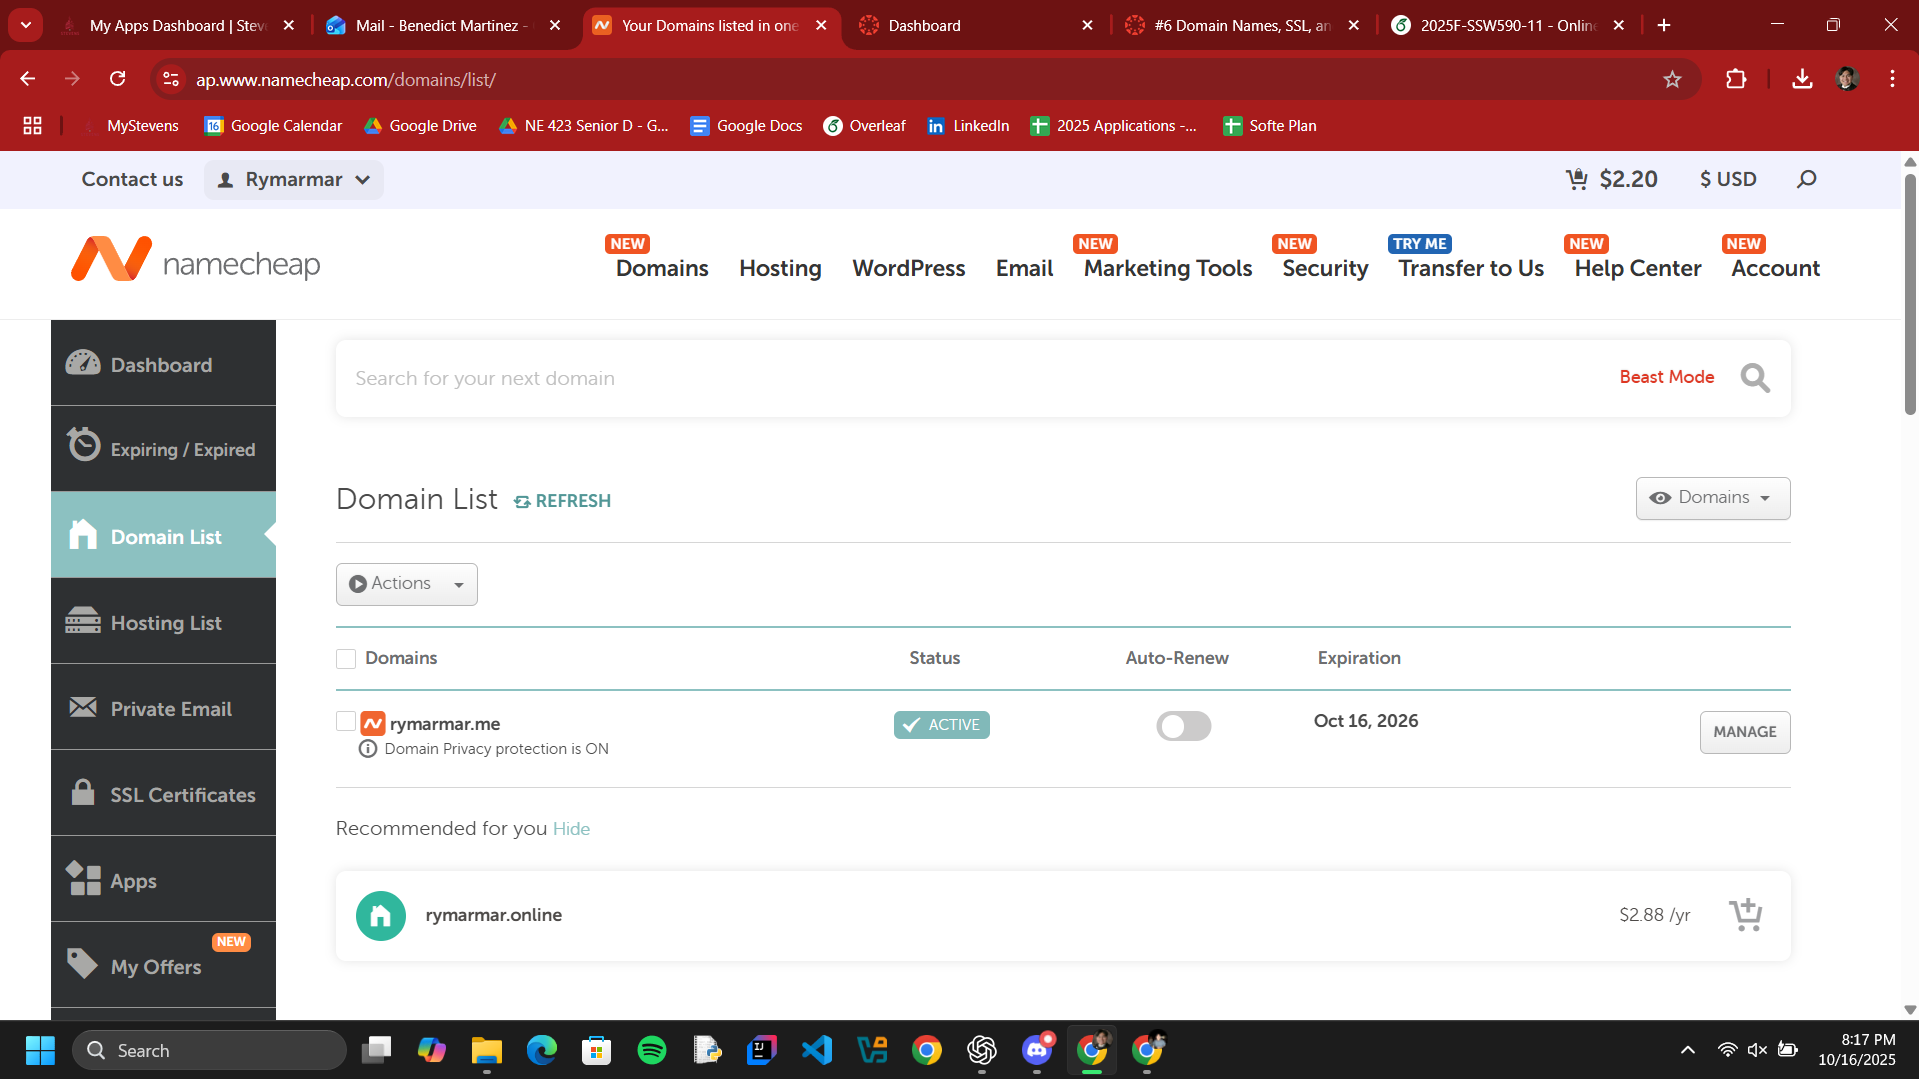
\includegraphics[width=\textwidth]{png/DomainNames/domain_list.png}
%     \caption{Namecheap domain list confirming registration of \texttt{rymarmar.me}.}
% \end{figure}

%----------------------------------------------------
% \section{Step 2: SSL Certificate Configuration}
% To secure all traffic, we enabled \textbf{HTTPS enforcement} using GitHub Pages, which automatically provisions SSL certificates through Let’s Encrypt (renewed every 90 days).  
% This provides secure HTTPS access without needing to manually install certificates.

% \begin{figure}[H]
%     \centering
%     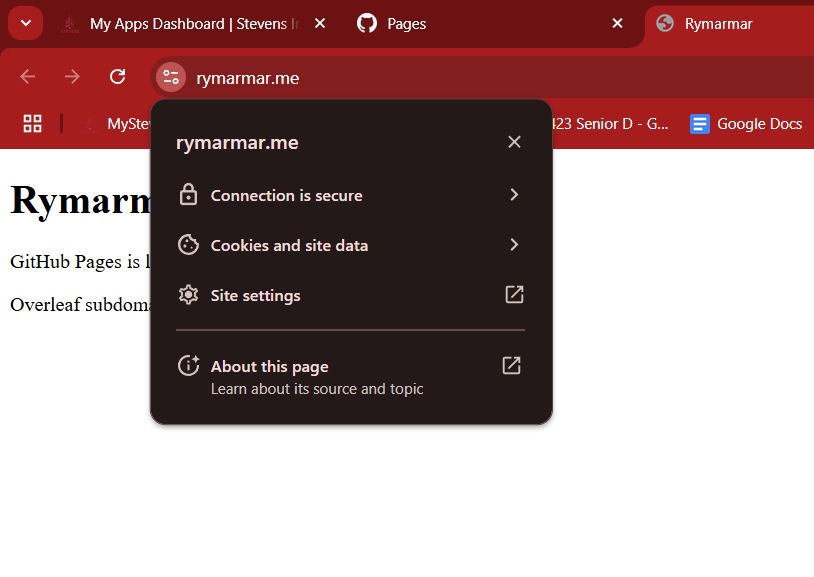
\includegraphics[width=\textwidth]{png/DomainNames/Enforce_HTTPS.png}
%     \caption{GitHub Pages settings showing HTTPS enforcement and DNS verification.}
% \end{figure}

% \begin{figure}[H]
%     \centering
%     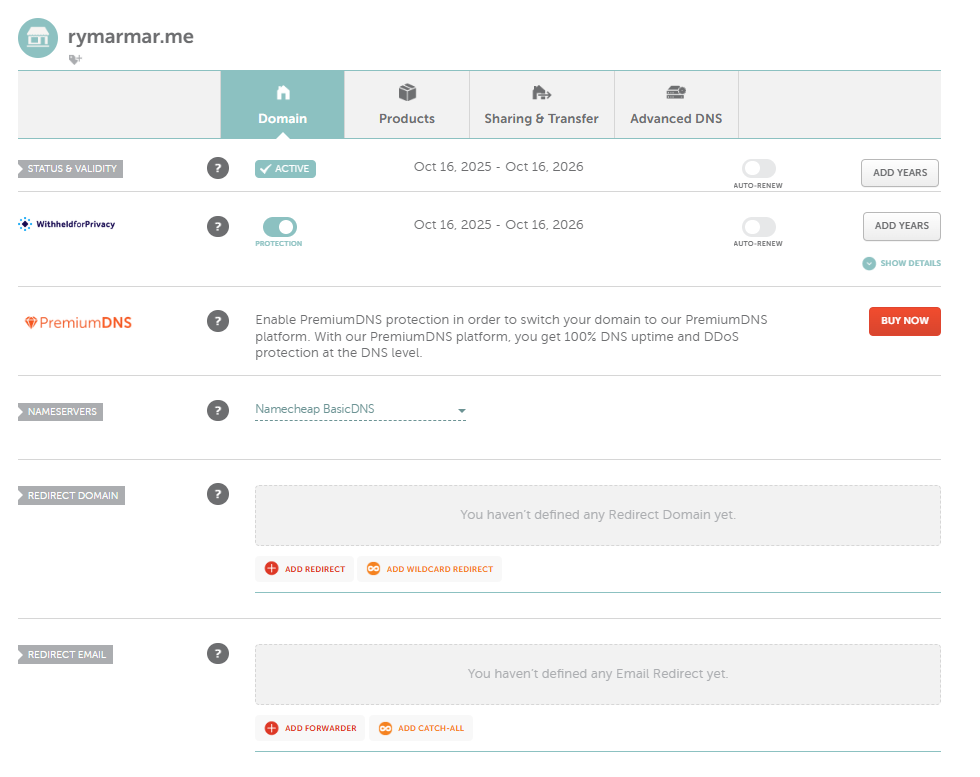
\includegraphics[width=0.7\textwidth]{png/DomainNames/domain_secured.png}
%     \caption{Browser confirmation that \texttt{https://rymarmar.me} is secured via SSL.}
% \end{figure}

% \begin{figure}[H]
%     \centering
%     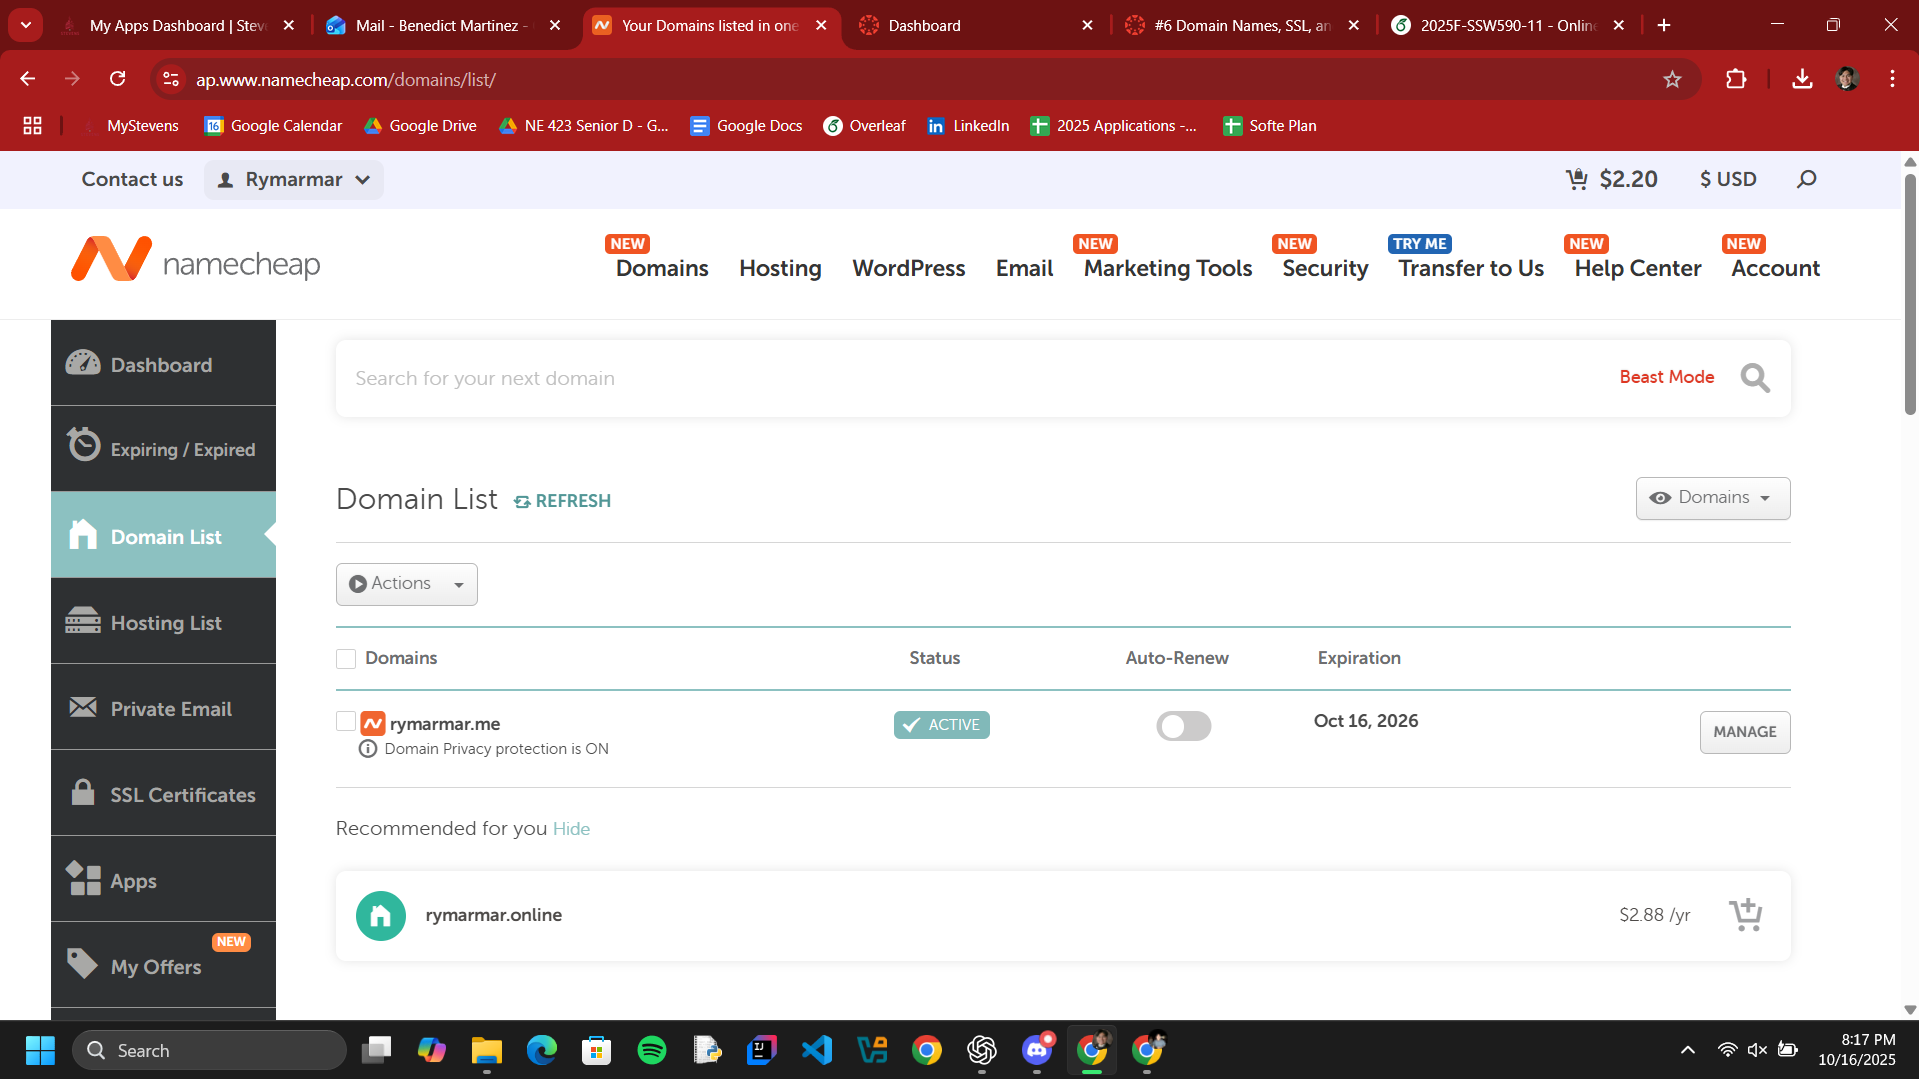
\includegraphics[width=\textwidth]{png/DomainNames/domain_list.png}
%     \caption{Namecheap domain list confirming registration of \texttt{rymarmar.me}.}
% \end{figure}
%----------------------------------------------------
\section{SSL Configuration}

The choice we made for providing SSL to the domain is using Let's Encrypt.
\begin{minted}{Bash}
# Install Certbot
apt install -y certbot python3-certbot-nginx

# Stop Overleaf temporarily
cd /opt/overleaf/toolkit
bin/stop

# Get SSL certificate (replace with your domain)
certbot certonly --standalone -d your-domain.com

# Update config/overleaf.rc
OVERLEAF_SITE_URL=https://your-domain.com
OVERLEAF_PORT=443

# Configure SSL in config/overleaf.yml
# Then restart
bin/start
\end{minted}
% We created a Caddyfile and modified the docker-compose file.    
% \begin{figure}[H]
% \begin{minted}[linenos]{python}
%      1	services:
%      2	    sharelatex:
%     16	        volumes:
%     33	            OVERLEAF_SITE_URL: "https://ssw590team11.me"
%    156	    caddy:
%    157	      image: caddy:latest
%    158	      container_name: caddy
%    159	      ports:
%    160	        - "80:80"
%    161	        - "443:443"
%    162	      volumes:
%    163	        - ./Caddyfile:/etc/caddy/Caddyfile
%    164	        - caddy_data:/data
%    165	        - caddy_config:/config
%    166	      depends_on:
%    167	        - sharelatex
%    168	      restart: unless-stopped
%    169	volumes:
%    170	  mongo_data:
%    171	  caddy_data:
%    172	  caddy_config:
% \end{minted}
% \caption{docker-compose.yml additions}
% \end{figure}

% \begin{figure}[H]
% \begin{minted}[linenos]{python}
% ssw590team11.me {
% 	reverse_proxy sharelatex:80
% }
% \end{minted}
% \caption{Caddyfile}
% \end{figure}

% We also added records on Digital Ocean and Namecheap to link our droplet to the domain.

% \begin{figure}[H]
%     \centering
%     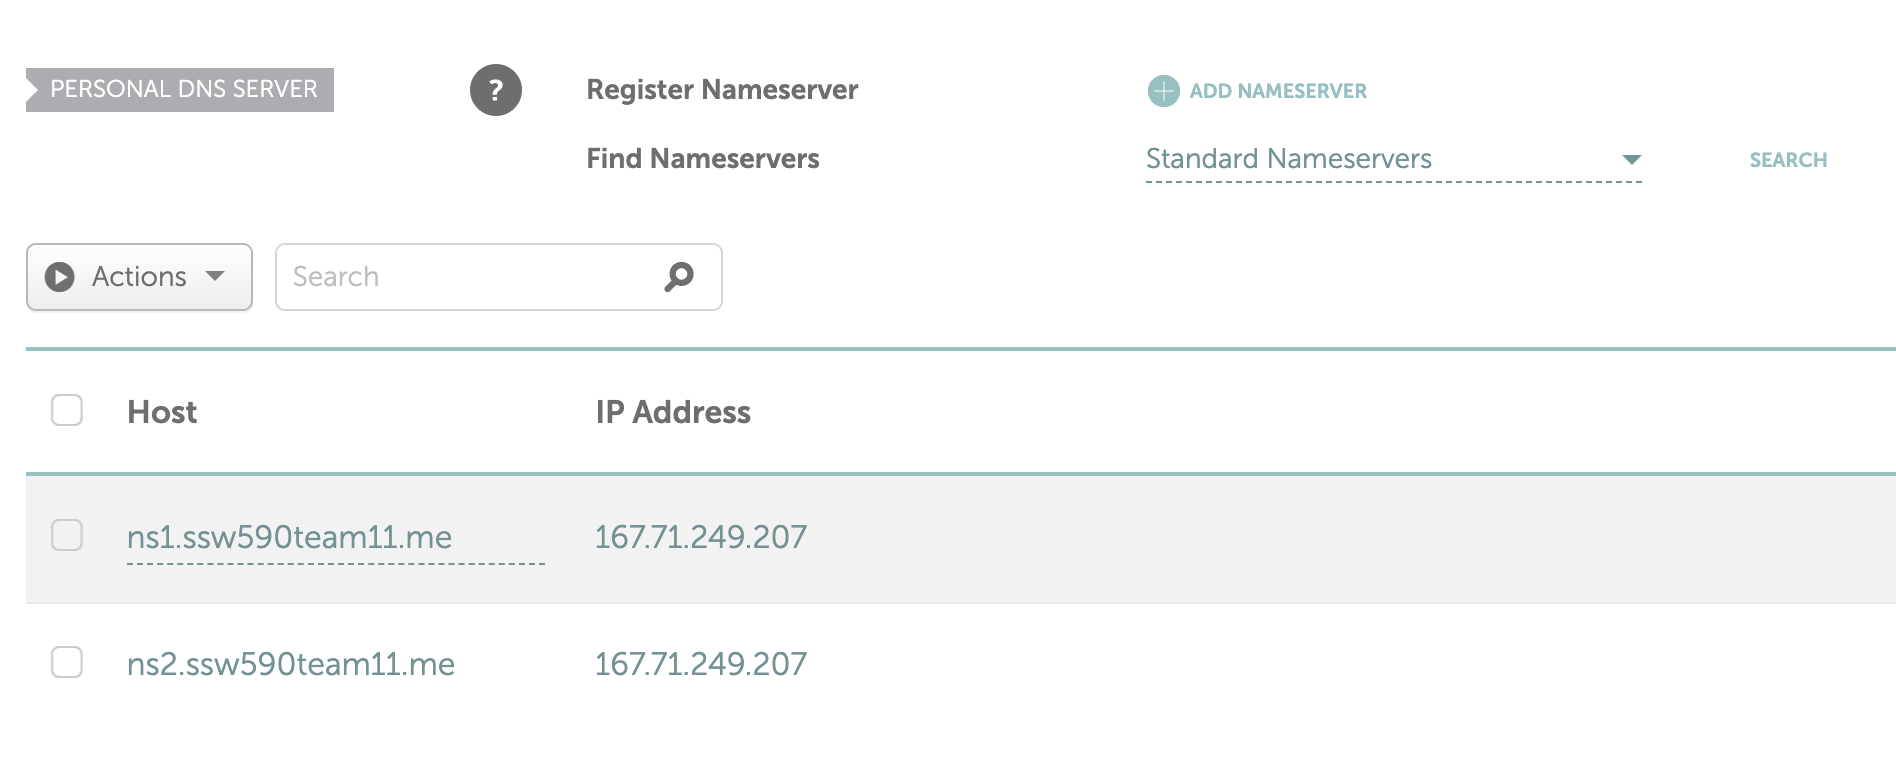
\includegraphics[width=0.7\textwidth]{png/DigitalOcean/DigitalOceanDNS.png}
%     \caption{Digital Ocean DNS records linking to domain}
% \end{figure}

% \begin{figure}[H]
%     \centering
%     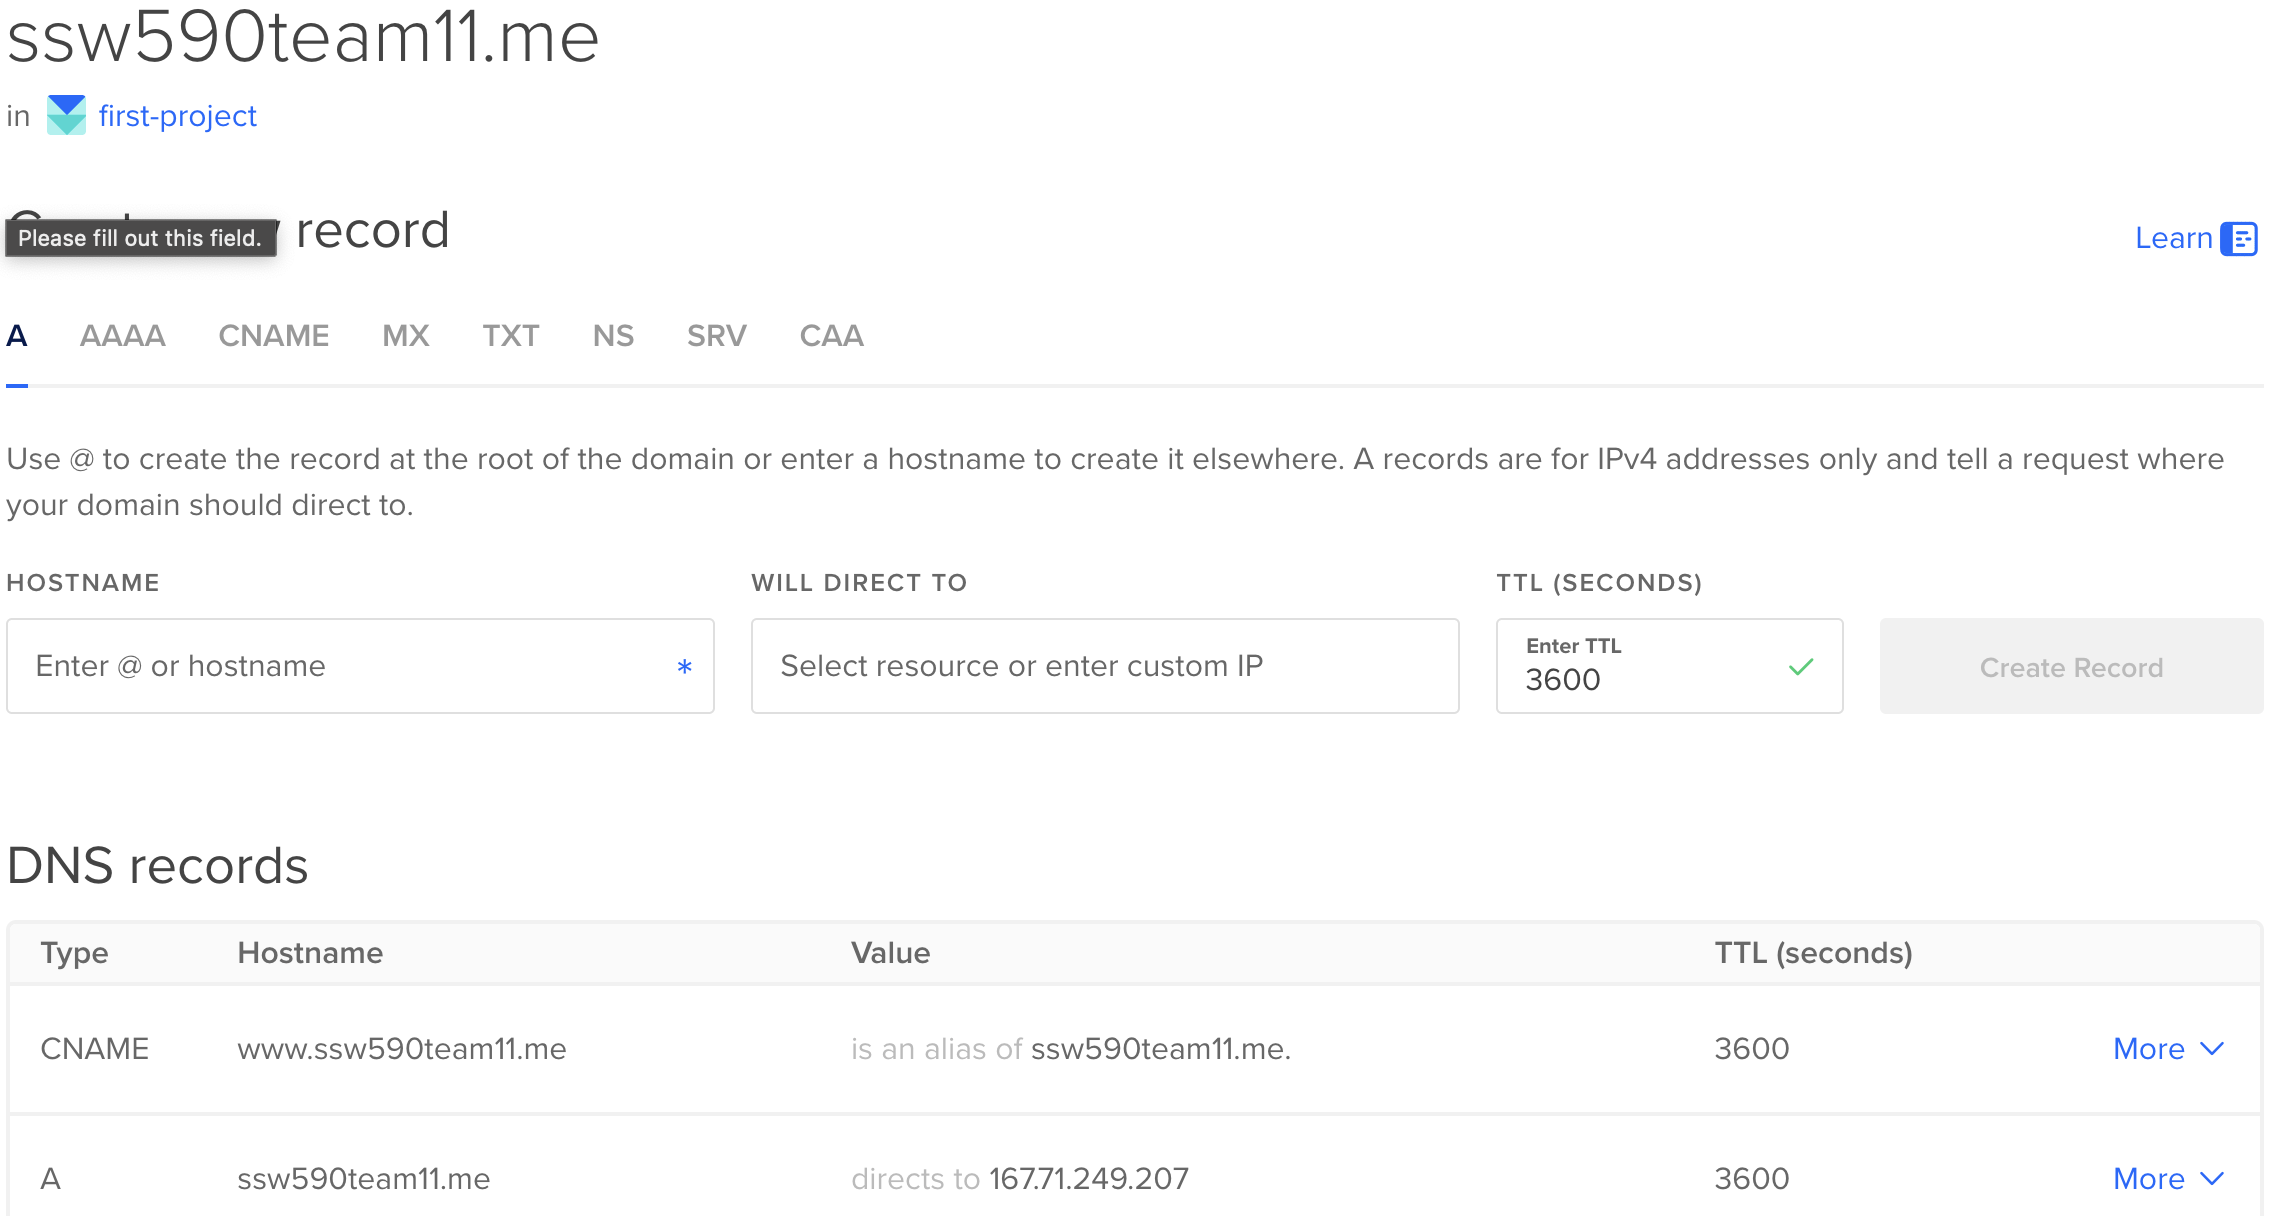
\includegraphics[width=0.7\textwidth]{png/DigitalOcean/NamecheapRecords.png}
%     \caption{Namecheap DNS records to go to droplet IP address}
% \end{figure}

%----------------------------------------------------
% \section{Step 3: Overleaf Container Setup on DigitalOcean}
% Our teammates (Charles and Justin) deployed an Overleaf Community Edition container using a DigitalOcean droplet.  
% This ensured the Overleaf instance supported all LaTeX packages and allowed testing of compilation consistency.  
% The container was connected to our team GitHub repository and included a custom domain mapping for the subdomain.

% \begin{minted}{bash}
% # Example Docker-based deployment used on DigitalOcean
% sudo docker run -d --name overleaf -p 80:80 sharelatex/sharelatex
% \end{minted}

% This step satisfied the “configure container/image” requirement for Overleaf hosting.  
% The configuration process was documented and replicated locally for testing.

% \begin{figure}[h!]
%     \centering
%     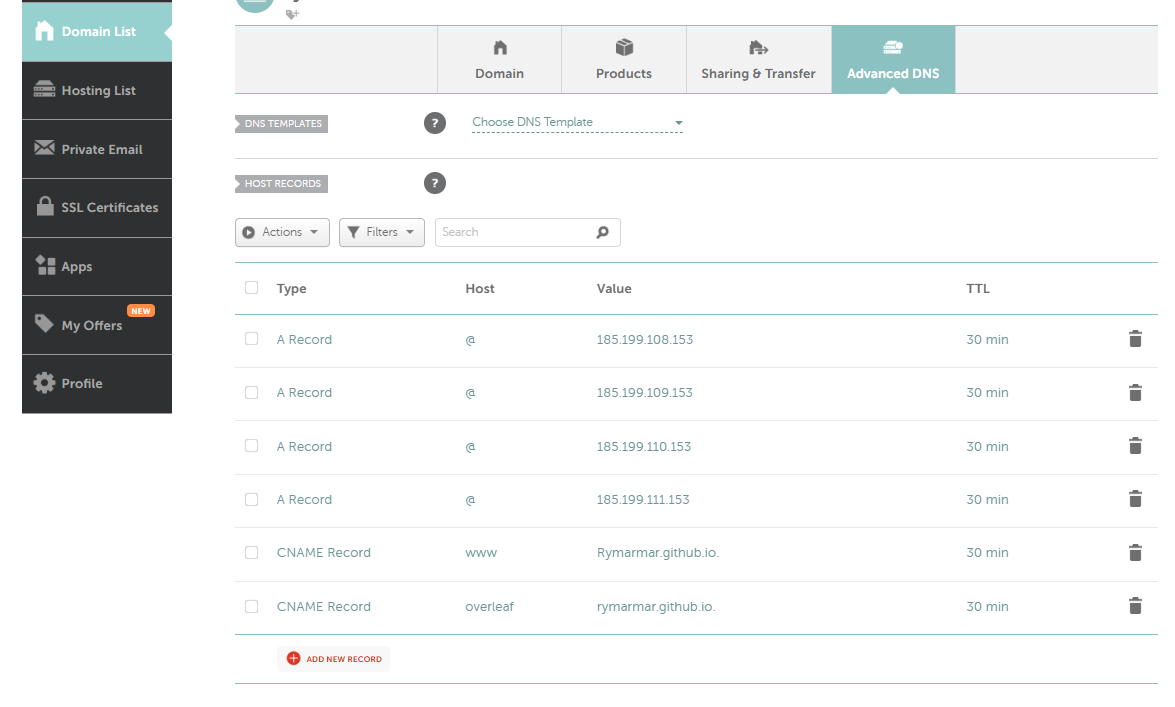
\includegraphics[width=\textwidth]{png/DomainNames/namespacesettings.png}
%     \caption{Namecheap Advanced DNS configuration showing A and CNAME records for the root and subdomains.}
% \end{figure}

% \begin{figure}[h!]
%     \centering
%     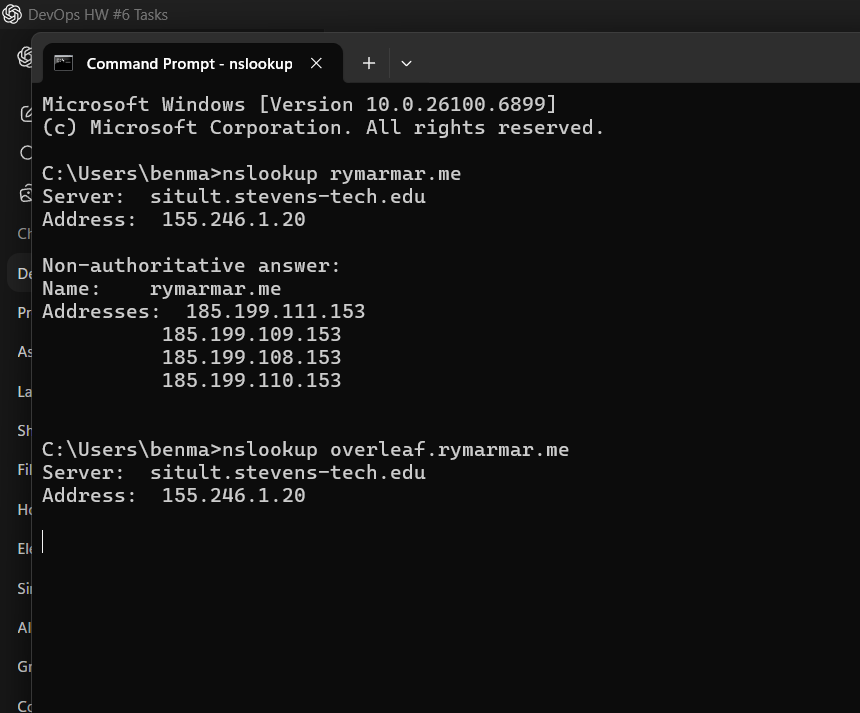
\includegraphics[width=0.85\textwidth]{png/DomainNames/cmd_checkup.png}
%     \caption{Verification using \texttt{nslookup} confirming successful DNS and subdomain resolution.}
% \end{figure}

%----------------------------------------------------

\section{Overleaf Container LaTeX Packages Configuration}
\begin{itemize}
    \item In order for our Overleaf to support all LaTeX packages one might use in their document, the commands below must be used to install all LaTeX packages.
\end{itemize}
\begin{minted}{Bash}
bin/docker-compose exec sharelatex bash
tlmgr update --self 
tlmgr install scheme-full
\end{minted}
   
% \section{Step 4: GitHub Pages Integration (Benedict)}
% The GitHub repository \texttt{Rymarmar.github.io} was configured to serve as the main site using the custom domain \texttt{rymarmar.me}.  
% Deployment is configured directly from the \texttt{main} branch, and HTTPS is now enforced.  
% This serves as a simple landing page while the Overleaf container is being finalized.

% \begin{figure}[h!]
%     \centering
%     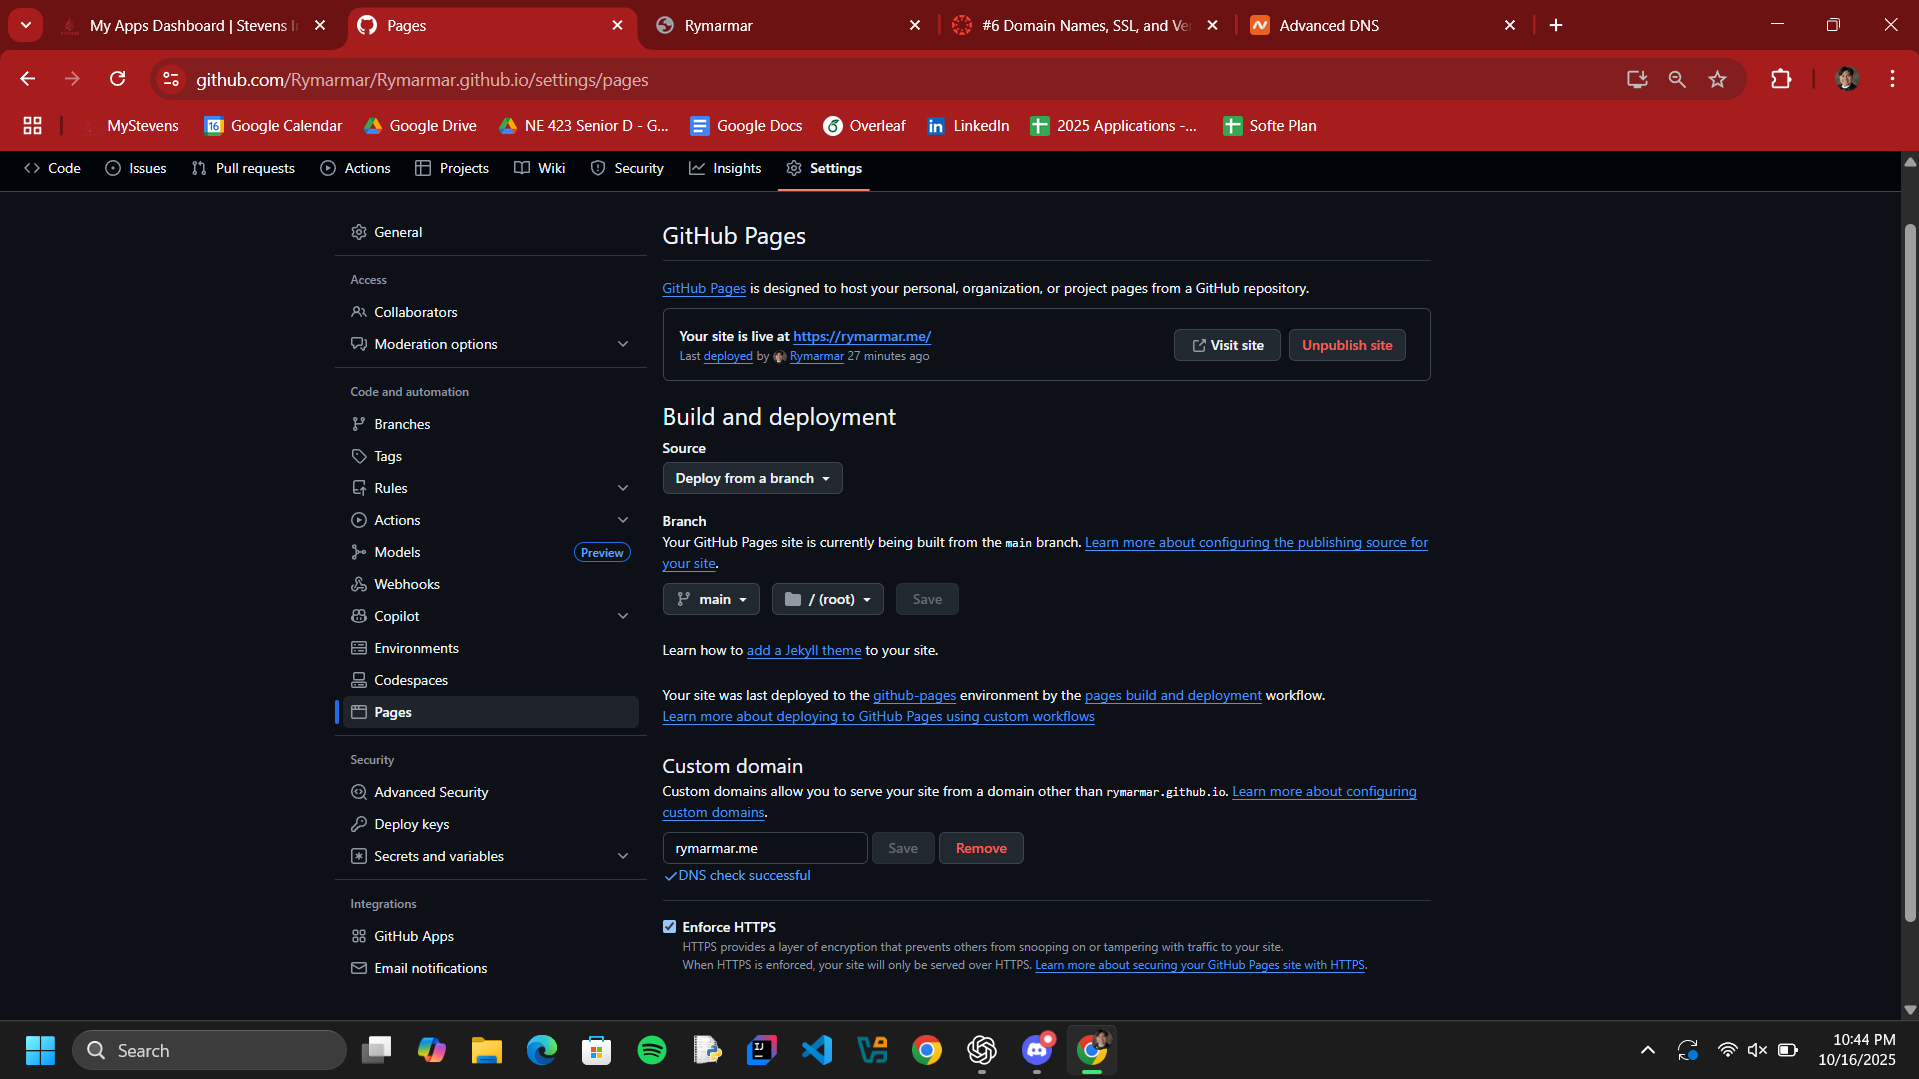
\includegraphics[width=\textwidth]{png/DomainNames/github settings.png}
%     \caption{GitHub Pages settings confirming DNS validation and HTTPS enforcement.}
% \end{figure}

% The \texttt{index.html} page was published successfully. Some users experienced delays when loading the domain due to DNS propagation time, but configuration remains correct.

% \begin{figure}[h!]
%     \centering
%     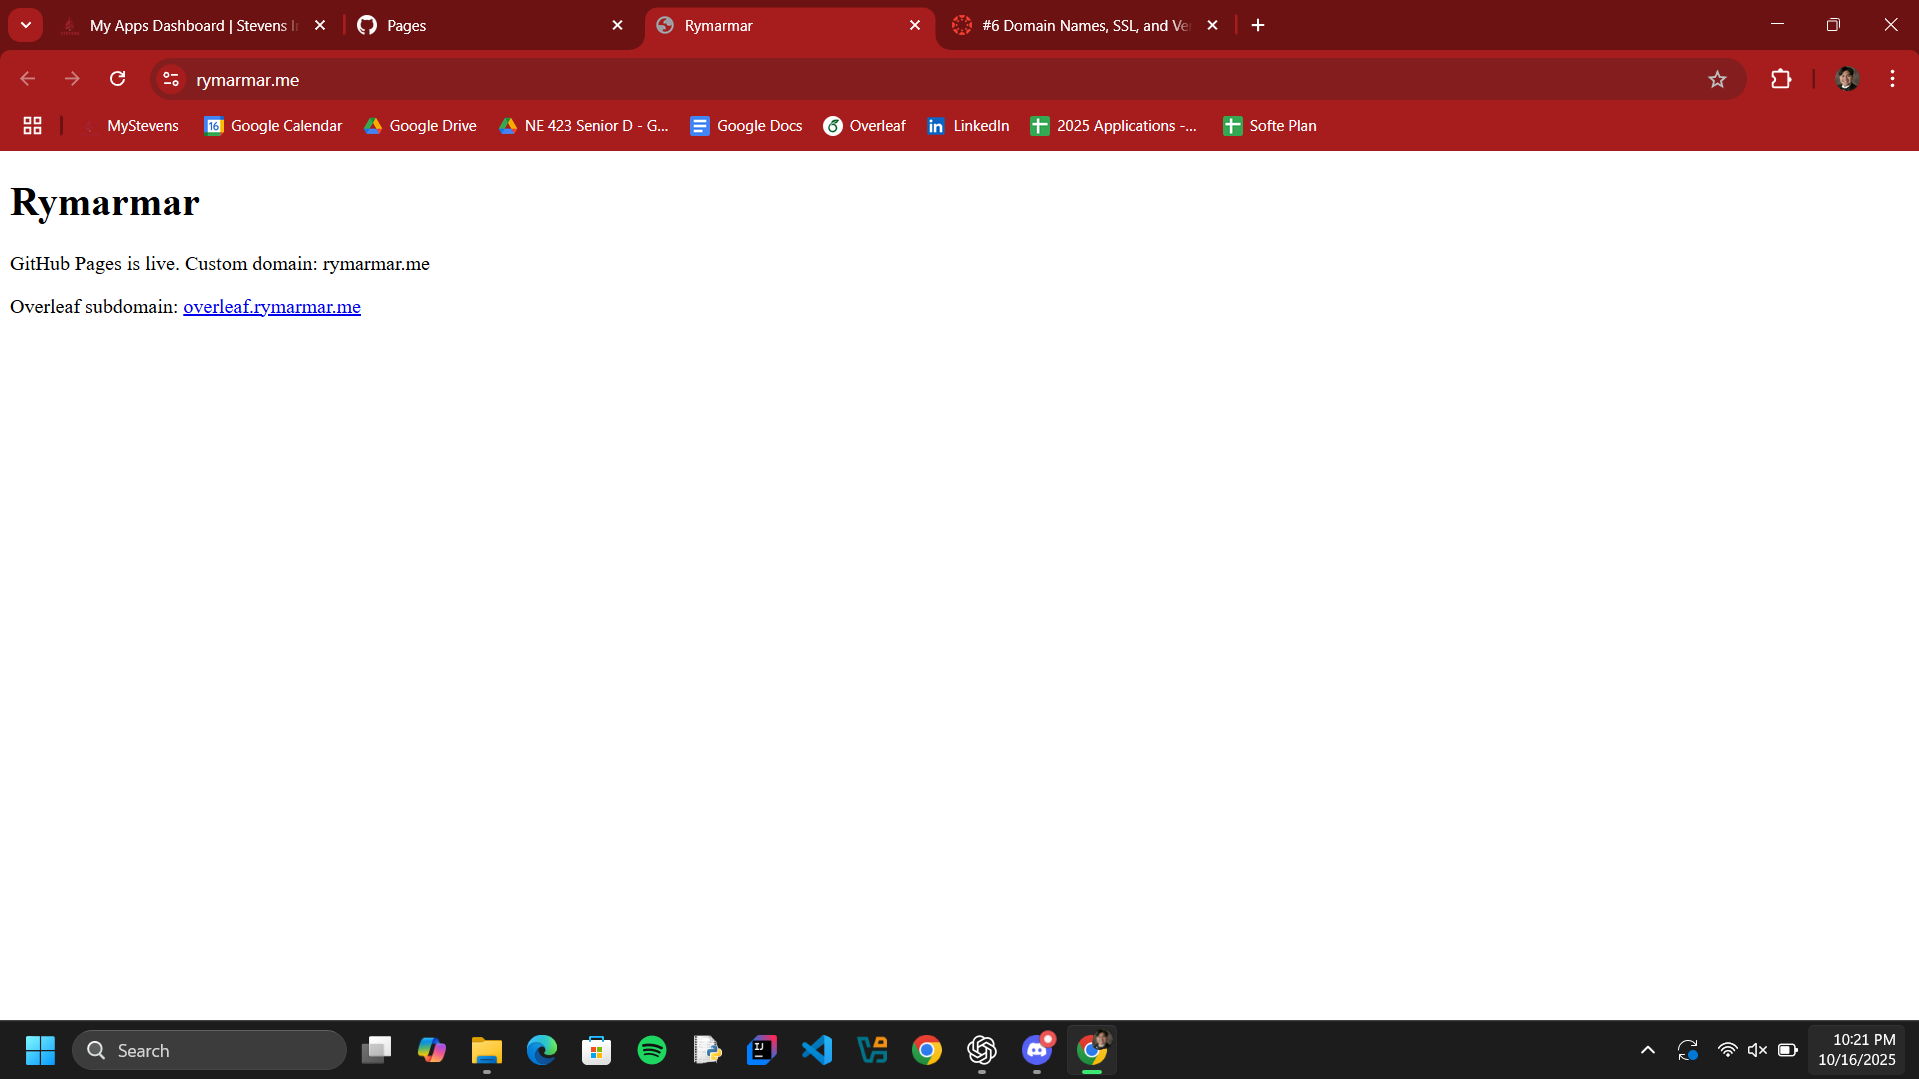
\includegraphics[width=\textwidth]{png/DomainNames/website.png}
%     \caption{Deployed GitHub Pages site confirming build and domain resolution for \texttt{rymarmar.me}.}
% \end{figure}

% %----------------------------------------------------
% \section{Step 5: Overleaf Subdomain Redirect Verification}
% A subdomain \texttt{overleaf.rymarmar.me} was created in Namecheap and configured to redirect to our GitHub Pages site.  
% This verifies that DNS records for the Overleaf subdomain resolve correctly.

% \begin{figure}[h!]
%     \centering
%     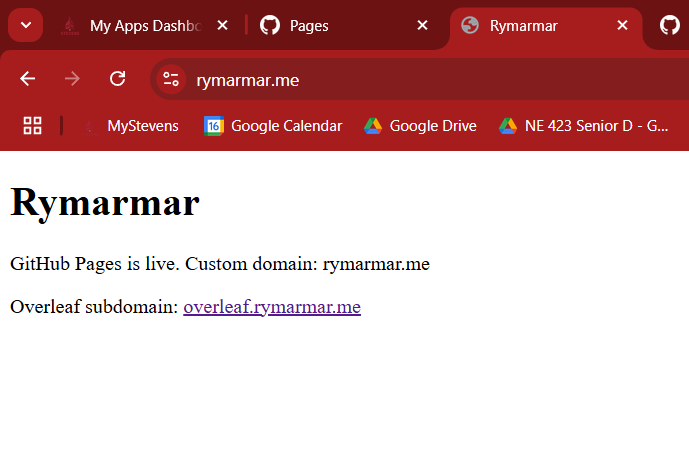
\includegraphics[width=\textwidth]{png/DomainNames/overleaf_redirect.png}
%     \caption{The subdomain \texttt{overleaf.rymarmar.me} redirecting to the main site \texttt{rymarmar.me}.}
% \end{figure}

%----------------------------------------------------
\section{Overleaf–GitHub Sync}
Overleaf’s paid Git integration feature is unavailable for free users, so synchronization is currently being replicated manually using Git commands.  
The workflow allows us to update Overleaf projects locally and push them to GitHub for version tracking. \\

\textbf{Repo: }\url{https://github.com/CharlesVilla68/Overleaf590.git}

\begin{enumerate}
    \item Head to the GitHub site and create a new repository
    \item Generated SSH key on the server
    \item Added the SSH key to GitHub
    \item Verified SSH connection to confirm that the server could communicate with GitHub
    \item Cloned the GitHub repository into the "/opt/latex-projects/" directory
    \item Downloaded the project from Overleaf as a ZIP file and uploaded it to the server using "scp"
    \item Committed and pushed to GitHub by extracting the files, staging them, and then committing/pushing to GitHub to sync everything
\end{enumerate}

\begin{itemize}
    \item We used these commands below in the terminal to create and push all the Overleaf files to the repository we created
\end{itemize}

\begin{minted}{Bash}
    git init 
    git remote add origin https://github.com/CharlesVilla68/Overleaf590.git
    git add . 
    git commit -m "First commit"
    git push -u origin main
\end{minted}

\section{Overleaf Project Local Compilation}
\begin{itemize}
    \item In order to compile our Overleaf project locally, we used these commands below.
\begin{minted}{Bash}
cd /opt/overleaf/toolkit
bin/docker-compose exec sharelatex bash -c "mkdir -p /tmp/compile && rm -rf /tmp/compile/*"
bin/docker-compose cp /opt/latex-projects/Overleaf590/2025F_SSW590_11/. sharelatex:/tmp/compile/
bin/docker-compose exec sharelatex bash -c "cd /tmp/compile && pdflatex -interaction=nonstopmode itManual.tex"
bin/docker-compose cp sharelatex:/tmp/compile/itManual.pdf /opt/latex-projects/Overleaf590/2025F_SSW590_11/
ls -lh /opt/latex-projects/Overleaf590/2025F_SSW590_11/itManual.pdf
scp root@159.65.44.227:/opt/latex-projects/Overleaf590/2025F_SSW590_11/itManual.pdf ./
\end{minted}
\end{itemize}

\begin{figure}[htp]
    \centering
    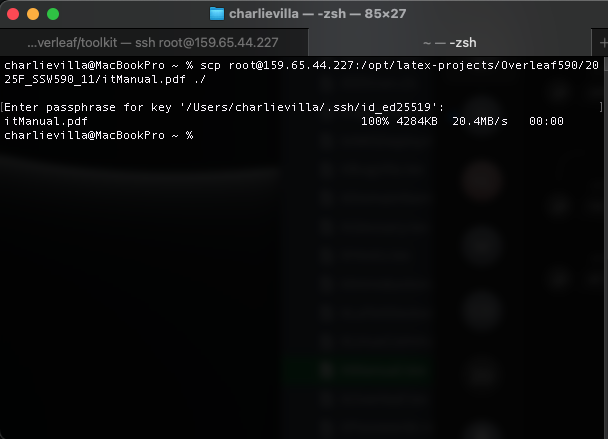
\includegraphics[width=15cm, height=10cm]{png/DomainNames/CL Compiling Pic.png}
    \caption{After Compiling in Command Line}
    \label{fig:DomainNames}
\end{figure}

%----------------------------------------------------
\section{GitHub Version Hash Key Titling}
To map each document version to a Git commit, versioning will be added to the document title once the sync process is finalized. This ensures full traceability between the Overleaf PDF and the GitHub repository version.

\begin{enumerate}
    \item Retrieved the commit hash by using "git log -1 --format=\%h" to get the short version of the latest GitHub commit hash
    \item Modified the LaTeX title to include the commit hash in the document title
    \item Recompiled and pushed the updated LaTeX file to GitHub
\end{enumerate}

% \begin{minted}{latex}
% \title{SSW 590 - Domain Names, SSL, and Versioning (v1.0 - Commit 6fdbbf1)}
% \end{minted}



%----------------------------------------------------
% \section{Conclusion and Deliverable Checklist}
% This assignment demonstrates the end-to-end setup of a secured domain with SSL, integration with GitHub Pages, and configuration for an Overleaf instance hosted on DigitalOcean.  
% Minor remaining work includes automating Overleaf <-> GitHub syncing and embedding commit hashes in titles for traceability.

% \begin{itemize}
%     \item[1.] \textbf{Domain Name:} Registered \texttt{rymarmar.me} via GitHub Student Pack – \checkmark
%     \item[2.] \textbf{SSL Configuration:} HTTPS enforced via GitHub Pages / Let’s Encrypt – \checkmark
%     \item[3.] \textbf{Overleaf Container Setup:} Hosted on DigitalOcean droplet – \checkmark
%     \item[4.] \textbf{GitHub Pages Integration:} Site deployed and DNS verified – \checkmark
%     \item[5.] \textbf{Overleaf Subdomain Redirect:} Verified redirect to GitHub Pages – \checkmark
%     \item[6.] \textbf{Overleaf <-> GitHub Sync:} Manual workflow setup – \textit{In Progress}
%     \item[7.] \textbf{Version/Hash in Title:} Format added, implementation pending – \textit{In Progress}
% \end{itemize}
